%!TEX root = ../pres.tex

\begin{frame}
  \frametitle{Problem: ML for Pacman.}
  \begin{columns}
    \begin{column}{0.5\textwidth}

    \onslide<1->{
    \emph{How would you solve pacman with machine learning?} } \\[0.9cm]

    \onslide<2->{
   \textbf{ Find a model which takes screen pixels to actions:}
    \begin{equation*}
      \pi_\theta: s_t \mapsto a_t.
    \end{equation*}}

    \onslide<3->{
      \emph{What is your loss function? Data?}
    }
   
    \end{column}
    \begin{column}{0.5\textwidth}
    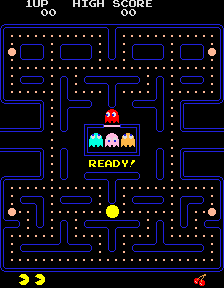
\includegraphics[width=0.9\textwidth]{Pac-man.png}
    \end{column}
  \end{columns}
\end{frame}


\begin{frame}
  \frametitle{Problem: ML for Pacman.}
  \begin{columns}
    \begin{column}{0.5\textwidth}
    \begin{equation*}
    \ugearrow
    \end{equation*}
    \end{column}
    \begin{column}{0.5\textwidth}
    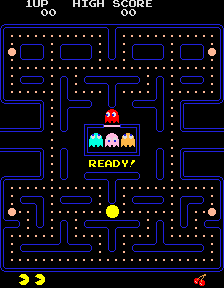
\includegraphics[width=0.9\textwidth]{Pac-man.png}
    \end{column}
  \end{columns}
\end{frame}




\begin{frame}
  \frametitle{Solution: Reinforcement Learning}
  \begin{columns}
    \begin{column}{0.5\textwidth}
      \begin{itemize}
        \item<1-> Supervised learning is \emph{not} the most general formulation of learning.
        \item<2-> Humans learn through reward and penalty
      \end{itemize}
    \end{column}
    \begin{column}{0.5\textwidth}
    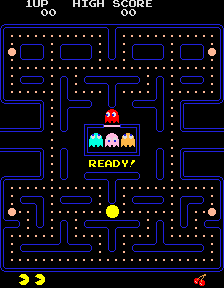
\includegraphics[width=0.9\textwidth]{Pac-man.png}
    \end{column}
  \end{columns}
\end{frame}


\begin{frame}
  \frametitle{Solution: Reinforcement Learning}
  \begin{columns}
    \begin{column}{0.5\textwidth}
      \begin{itemize}
        \item<1-> Can we make algorithms which improve with crude reward signals?
      \end{itemize}
       \begin{center}
        \textbf{Machine learning without explicit objective functions}
        \begin{equation*}
        	\Downarrow
        \end{equation*}
        \textbf{Reinforcement Learning (RL)}
        \end{center}
    \end{column}
    \begin{column}{0.5\textwidth}
    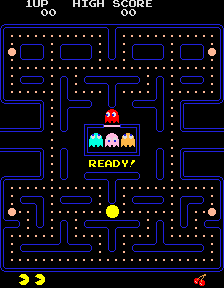
\includegraphics[width=0.9\textwidth]{Pac-man.png}
    \end{column}
  \end{columns}
\end{frame}
